\chapter{Loudness}
\label{Loudness}
\noindent
\textit{Loudness} er et omdiskuteret emne og et effektivt værktøj som påvirker mennesker på forskellig vis. Baggrundsstøj er så påtrængende i hverdagsomgivelser at det er svært at finde stillesoner, og det høje lydtryksniveau øger risikoen for høreskader, \parencites[ss. 1-2]{BOOK:Loudness}. Mennesker afhænger af den auditive sans til at færde sig i sine omgivelser og skærpe opmærksomheden i farlige situationer, hvorfor vi reagerer kraftigt på høje lyde. Dette kan udnyttes til mere eller mindre noble formål, eksempelvis kan en bilist benytte hornet til advare en forbipasserende for at undgå en ulykke, men det kan også benyttes i reklameindustrien hvor lydtryksniveauet kan øges for at fange potentielle købers opmærksomhed, \parencite[s. 3]{BOOK:Loudness}. For at undgå at radio- og TV-reklamer lyder væsentligt højere end det resterende indhold, er der indført anbefalinger og regulationer for \textit{Programme Loudness}, \textit{Loudness Range} og \textit{Maximum True Peak Level}, som forholder sig til \textit{Loudness} på forskellig vis. \parencite{STD:R108}.
\blankline
Også musikproducenter gør brug af \textit{Loudness}, hvorfra termen \textit{Loudness War} er opstået. Det går i alt sin enkelthed ud på at pladeselskaber øger lydtryksniveauet i et stykke musik med dynamisk kompression og \textit{limiting}. Metoderne som er ens, men af forskellig omfang og effekt, reducerer dynamisk variation i musikken og øger samtidig RMS-niveauet, \parencite[s. 1177]{PDF:QualityAndLoudnessJudgements}.\par
At øge lydtryksniveauet er et effektivt værktøj til at fange opmærksomheden og ifølge \textcite[s. 3]{PDF:TheSeductiveAppealofLoudMusic} kan høje lydtryksniveauer betragtes som værende en \textit{space transporter}, fordi lytteren bliver funktionelt døv overfor det omkringværende miljø. Af samme årsag lytter professionelle musikere og lydteknikere ved højt lydtryksniveau fordi det tillader dem at høre flere nuancer, mens de producerer musikken. I den sammenhæng kan dynamik være et problem, fordi den samme forstærkning, som gør de lave passager i en sang høje nok, til at lydteknikere kan høre detaljerne, samtidig forstærker de høje passager til lydtryksniveauer som kan være skadelige, \parencite[s. 4]{PDF:TheSeductiveAppealofLoudMusic}. Dette kan være med til at forklare incitamentet til at producere musik med lav dynamik, som fylder hele amplituden af formatet. Et andet er at ifølge \textcite{WEB:LoudnessWarSecret} så hersker der en fejlagtig idé i brancen om at dynamisk komprimeret musik sælger bedre, fordi det fanger lytteres opmærksomhed. \textcite{WEB:LoudnessWarSecret} argumenterer samtidig for at effekten udlignes når alle kunstnere hæver lydtryksniveauet, i hvilket tilfælde musik med høj dynamik faktisk har en bedre chance for at udskille sig fra mængden, fordi det i sidste ende er lytteren, der bestemmer lydtryksniveauet for afspilningen med en volumenkontrol. Dynamisk komprimeret musik og i særdeleshed musik, som har været udsat for \textit{limitting}, har i øvrigt den ulempe at det udover at få forstærket de lave passager, kan miste kontrast og dybdefølelse, \parencite{WEB:WhatIsTheLoudnessWar}.
\blankline
Med den udvikling i musikindustrien og et estimat af at 1.1 millarder teenagere og unge voksne (mellem 12-35 år) er i risiko for høretab grundet usikker brug af personlige auditive enheder samt en skadelig støjbelastning på spillesteder, \parencite{WEB:WHOHearingLoss}, vil det være gavnligt, blandt andet at ændre folks lyttevaner. Hvis det er muligt at høre musik ved lavere lydtryksniveauer uden at opgive detaljerne i lydbilledet, kunne det muligvis øge lytteres incitament til at lytte til musik ved lavere lydtryksniveauer. 
\blankline
Denne rapport vil forsøge at klarlægge og analysere hvordan vi perciperer lyd afhængigt af frekvens og lydtryksniveau, samt udvikle en teknologisk løsning, der sikrer at perceptionen af lyd, ikke ændres afhængigt af hvilket lydtryksniveau den afspilles ved. Det gøres med henblik på at gøre det mere attraktivt at sænke lydtryksniveauet ved musikafspilning. Inden da er det nødvendigt at definere hvad \textit{Loudness} er.
\blankline
\textit{Loudness} defineres, ifølge \textcite[s. 82]{PDF:FletcherMunson}, som værende en psykologisk term, der beskriver størrelsen af en auditiv sensation. Ifølge \textcite[s. 3]{BOOK:Loudness} rangeres \textit{Loudness} fra meget svag til meget kraftig, hvilket \textcite[s. 82]{PDF:FletcherMunson} argumenterer imod, da disse termer afhænger af oplevelsen, evnen til at percipere auditive stimuli og af personen der benytter termerne. Så når \textit{Loudness} måles, skal der foruden de fysiske karakteristika af en lyd, også tages højde for lytterens psykologiske- og fysiske tilstand. \textit{Loudness} bedømmes blandt andet ud fra hukommelse, multisensoriske interaktioner, tværkulturelle forskelle, baggrundstøj og måden hvorpå lyden præsenteres og måles, \parencite[ss. 4-5]{BOOK:Loudness}. Dertil skal der tages højde for at perception af \textit{Loudness} ved en bestemt hændelse ændres over tid, grundet sensoriske og kognitive faktorer, \parencite[s. 5]{BOOK:Loudness}. Ydermere skal der, ifølge \textcite[s. 82]{PDF:FletcherMunson}, tages højde for hvilket øre der registrer lyden samt lytterens opmærksomhed, årvågenhed og udmattelse. Udmattelse kan forekomme hvis en person har været eksponeret for lyde med høje lydtryksniveauer, hvilket vil resultere i at perceptionen af \textit{Loudness} ændres, \parencite[s. 6]{BOOK:Loudness}. Da bedømmelsen af \textit{Loudness} kan variere fra person til person, forefindes der ikke én bestemt objektiv metode til at måle \textit{Loudness}, \parencite[s. 4]{BOOK:Loudness}.
\blankline
Når \textit{Loudness} bedømmes kan det gøres ud fra enheden sone. Én sone er defineret som den perciperede \textit{Loudness} af en 1000Hz tone ved 40dB SPL, hørt binauralt i et frit felt, hvor lydkilden er placeret i lytterens frontale plan, \parencite[s. 4]{BOOK:Loudness}. SPL angiver \textit{Sound Pressure Level}, svarende til lydtryksniveau. Det vil fremover være indforstået at lydtryksniveauer angives i dB, medmindre andet specificeres. At målingerne foretages i et frit felt, betyder at de omkringværende objekter ikke reflekterer lyden. Der er et lineært forhold mellem sone og \textit{Loudness}, så en fordobling i sone resulterer i en fordobling af \textit{Loudness}. Derfor perciperes en tone med to sone som værende dobbelt så kraftig, som en 1000Hz tone ved 40dB, \parencite[s. 4]{BOOK:Loudness}.
\blankline
En anden måde at bedømme \textit{Loudness} på er ved brug af \textit{Loudness Level}, som, ifølge \textcite[s. 2]{STD:ISO226}, defineres til at være en værdi i phon, der har den samme numeriske værdi som lydstryksniveauet i dB tilhørende en referencetone. Hvor referencetonen består af en frontal hændelse; sinusformet progressiv plan bølge med en frekvens på 1000Hz, som vurderes til at være lige så høj, som en given lyd. Så hvis en tone eksempeltvist har et \textit{Loudness Level} på 60phon, resulterer det i at tonen lyder lige så kraftig som en 1000Hz tone ved 60dB. Ved 60phon skal en tone på 20Hz derfor have et lydtryksniveau på 109.5dB for at lyde lige så kraftig, som en 1000Hz ved 60dB, \autoref{app:ISO226Raadata}.
%
%Input kapitler her
\section{Equal-Loudness-Level Contours}
\label{Equal-loudness-level-contours}
Igennem de efterfølgende afsnit vil der blive givet en kort introduktion til tre af de mest betydningsfulde undersøgelser inden for \textit{Loudness}, hvor den sidste undersøgelse, \textcite{STD:ISO226}, danner grundlag for resten af rapporten. 
%
\subsection{Fletcher og Munson}
\label{Fletcher-Munson}
%
Den første undersøgelse af hvordan mennesket perciperer rene toner ved forskellige frekvenser i det hørbareområde, som går fra 20Hz til 20000Hz, blev foretaget af \textcite{PDF:FletcherMunson}. Sammenhængen mellem perceptionen af \textit{Loudness} for rene toner og frekvens blev målt på 11 forsøgspersoner, som alle udførte forsøget med høretelefoner på, \parencite[s. 86]{PDF:FletcherMunson}. Formålet var at måle et \textit{Loudness Level} ved at justere lydtryksniveauet af en referencetone, en ren tone på 1000Hz, så den lød lige så høj som den tone, den blev sammenlignet med, \parencite[s. 84]{PDF:FletcherMunson}. De toner som referencen blev sammenlignet med var i frekvensområdet 62Hz til 16000Hz, \parencite[s. 88]{PDF:FletcherMunson}. Resultatet af denne undersøgelse blev det første sæt \textit{Loudness-Level Contours}, og illustreres på \autoref{fig:FletcherMunson}.
%
\begin{figure}[H]
	\centering
	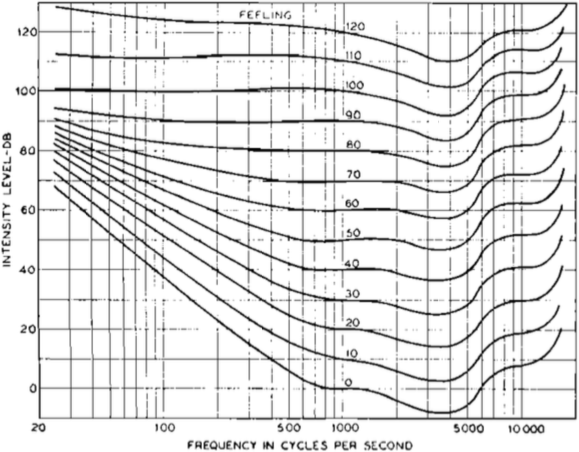
\includegraphics[resolution=300,width=\textwidth]{FletcherMunson}
	\caption{\textit{Loudness-Level Contours}, som blev udarbejdet af \textcite[s. 91]{PDF:FletcherMunson}. Hvor x-aksen angives som \textit{Frequency in cycles per second}, hvilket er den tidligere engelske betegnelse for frekvens i hertz, og y-aksen angiver lydtryksniveauer i dB.  Kurverne er angivet i værdier fra 0 til 120, med en stepsize på 10, og disse værdier svarer hver især til en specifik phon-kurve.}
	\label{fig:FletcherMunson}
\end{figure}
\noindent
%
Baseret på \autoref{fig:FletcherMunson} tyder det på at frekvenser under 1000Hz skal have et højere lydtryksniveau for at blive perciperet på samme måde, som referencetonen. Dog med forbehold for at ved høje lydtryksniveauer, over 80dB, udglattes kurverne, hvilket indikerer at lave frekvenser tilnærmelsesvist skal have det samme lydtryksniveau som referencen. Dykket ved samtlige kurver på \autoref{fig:FletcherMunson} skyldes at mennesker er mest sensitive overfor frekvenser i området fra 2000Hz til 5000Hz, \parencite{WEB:HowLoudIsTooLoud}.
\blankline
Ud fra den beskrevne eksperimentelle metode fremgår det at forsøget blev udført i et lydtæt rum, hvor forsøgspersonerne skulle vurdere om referencetonen var højere eller lavere end den tone der blev testet for, \parencite[s. 104]{PDF:FletcherMunson}. Derudover fremgår det, at der under forsøget var mere end én forsøgsperson inde i det lydtætte rum, \parencite[s. 104]{PDF:FletcherMunson}. Hver af de to forsøgspersoner skulle angive deres respons ved at trykke på nogle knapper, med henblik på at forsøgspersonernes respons således ikke ville påvirke hinanden, men det er uvist hvorvidt det har haft indflydelse på forsøgspersonernes respons at der var endnu en forsøgsperson i rummet. Dertil er undersøgelsen foretaget af \textcite{PDF:FletcherMunson} begrænset til kun at undersøge hvordan lyd perciperes igennem høretelefoner og er ikke foretaget i et frit felt, men i et lydtæt rum hvor høretelefonerne er kalibreret i forhold til rummet, så det giver effekten af et tilnærmelsesvist frit felt.\\
Grundet en stigende interesse på området blev der senere udført flere undersøgelser vedrørende mennesket perception af lyd, hvoraf en af dem er særligt nævneværdig; \textcite{PDF:RobinsonDadson}, som blev den første standard for \textit{Equal-Loudness Contours} og var den gyldige ISO226 indtil 2003. 
%
\newpage
\noindent
%
\subsection{Robinson og Dadson}
\label{Robinson-Dadson}
Undersøgelsen foretaget af \textcite[s. 166]{PDF:RobinsonDadson} er den første version af standarden ISO226, og beskriver forholdet mellem \textit{Equal-Loudness} og rene toner i et frit felt. Ligesom ved den førnævnte undersøgelse blev en ren referencetone på 1000Hz valgt til forsøget. Referencen blev sammenlignet med andre rene toner indenfor frekvensområdet fra 25Hz til 15000Hz og op til 130dB, \parencite[s. 167]{PDF:RobinsonDadson}. Undersøgelsen bygger på data indsamlet fra to grupper, hvor den ene gruppe bestod af 90 forsøgspersoner med begge køn ligeligt repræsenteret og et aldersspænd fra 16år til 63år. De deltog i omkring 30 forsøg. Den anden gruppe bestod af 30 forsøgspersoner, 17 mænd og 13 kvinder med en gennemsnitsalder på 30år, som deltog i over 100 forsøg, \parencite[s. 167]{PDF:RobinsonDadson}. Alle forsøgspersonerne der deltog i undersøgelsen blev forundersøgt for eventuelle høreskader og andre øresygdomme.\\
Forsøgspersonerne blev bedt om at vurdere hvilken af de to afspillede rene toner der var højest. Referencetonen var konstant 1000Hz men varierede i lydtryksniveau og den anden tone forblev konstant både i frekvens og lydtryksniveau, \parencite[s. 168]{PDF:RobinsonDadson}. Resultatet fra undersøgelsen fremgår af \autoref{fig:RobinsonDadson-Curves}.
%
\begin{figure}[H]
	\centering
	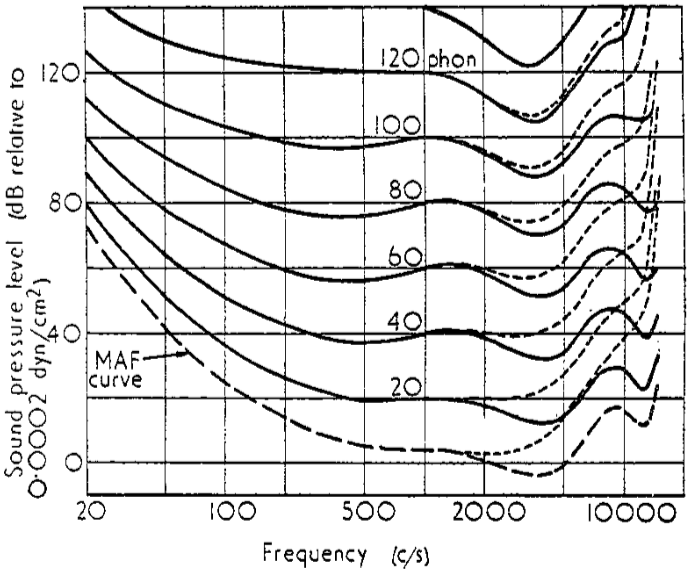
\includegraphics[resolution=300,width=\textwidth]{RobinsonDadson-Curves}
	\caption{\textit{Equal-Loudness Contours}, som blev udarbejdet af \textcite[s. 171]{PDF:RobinsonDadson}. X-aksen angiver frekvens i c/s, hvilket svarer til hertz og y-aksen angiver lydtryksniveauet. Kurverne er aldersopdelt, så de stiplede kurver repræsenterer aldersgruppen centreret omkring 60årige og kontinuerte kurver repræsenterer aldersgruppen centreret om 20årige forsøgspersoner.}
	\label{fig:RobinsonDadson-Curves}
\end{figure}
\noindent
%
\textcite[s. 171]{PDF:RobinsonDadson} fandt at ved frekvenser fra 25Hz til og med 1000Hz var der ingen aldersmæssig forskel, men fra 1000Hz og op forekom der en forskel, hvilket ligeledes fremgår af \autoref{fig:RobinsonDadson-Curves}.
\blankline
Ifølge \textcite[s. 918]{PDF:EqualLoudnessForPureTones} er der de senere år opstået ny interesse for \textit{Equal-Loudness-Level Contours} hvilket har resulteret i flere videnskabelige undersøgelser. Fælles for disse undersøgelser er, at de afviger fra resultaterne fundet af \textcite[s. 171]{PDF:RobinsonDadson}, særligt ved omkring 800Hz og ned hvor der måles et højere \textit{Equal-Loudness} niveau, \parencite[s. 918]{PDF:EqualLoudnessForPureTones}. Den store mængde af nye undersøgelser har været med til at danne grundlag for den nye, aktuelle standard; \textcite{STD:ISO226}.
%
\subsection{ISO226}
\label{ISO226}
%
I modsætning til både \textcite{PDF:FletcherMunson} og \textcite{PDF:RobinsonDadson} bygger \textcite[s. 9]{STD:ISO226} på 12 uafhængige videnskabelige undersøgelser, som alle lever op til følgende seks kriterier, fremsat i \textcite[s. 1]{STD:ISO226};
\blankline
\begin{alpherate}
  \item the sound field in the absence of the listener consists of a free progressive plane wave;
  \item the source of sound is directly in front of the listener;
  \item the sound signals are pure tones;
  \item the sound pressure level is measured at the position where the centre of the listener's head would be, but in the absence of the listener;
  \item listening is binaural;
  \item the listeners are otologically normal persons in the age range from 18 years to 25 years inclusive.
\end{alpherate}
\blankline
\noindent
%
Ydermere er frekvensområdet for de rene toner defineret til at være mellem 20Hz og 12500Hz, hvor frekvenserne vælges efter step af en tredjedel oktav. Resultaterne fra de 12 undersøgelser, som udgør \textcite{STD:ISO226}, er illustreret på \autoref{fig:EqualLoudnessContoursGraph} og går under navnet: \textit{Normal Equal-Loudness-Level Contours}.
%
\newpage
\noindent 
%
\begin{figure}[H]
	\centering
	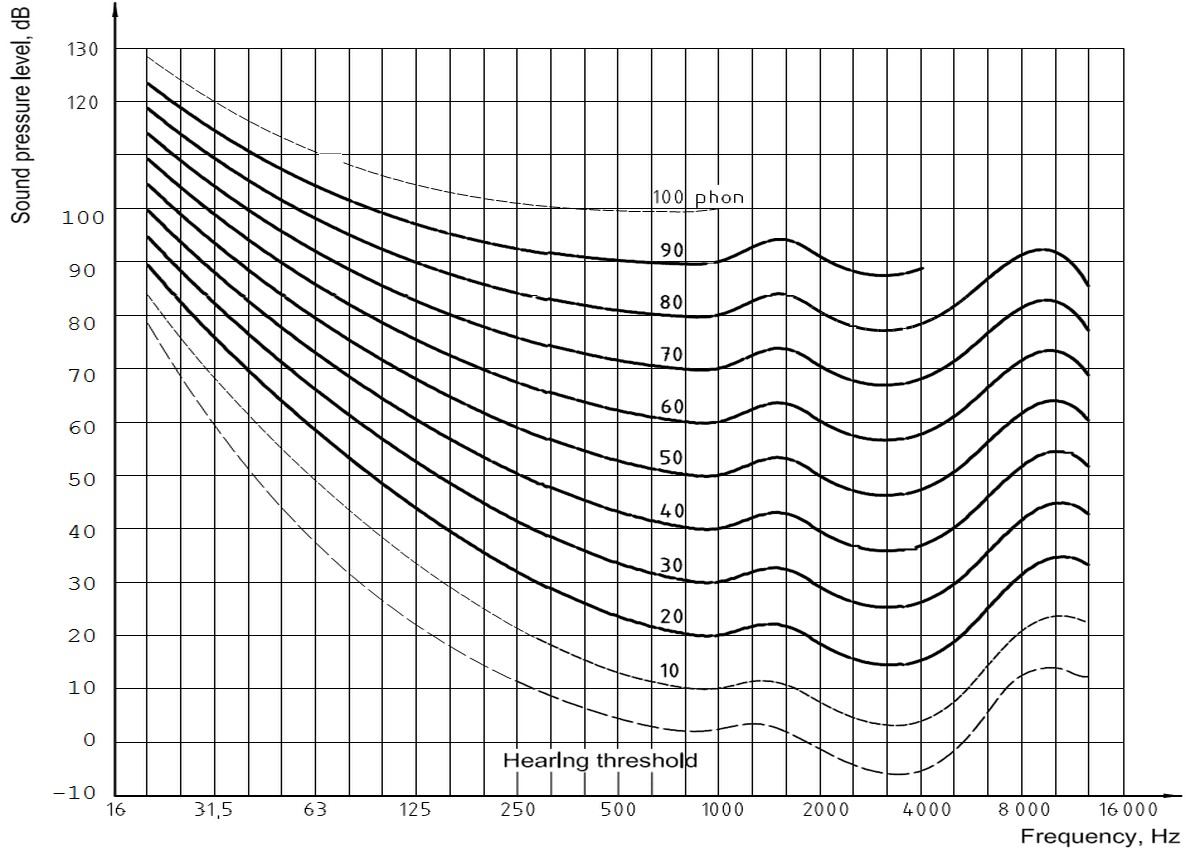
\includegraphics[resolution=300,width=\textwidth]{EqualLoudnessContoursGraph}
	\caption{\textit{Normal-Equal-Loudness-Level Contours} for rene toner fremsat i \textcite[s. 5]{STD:ISO226}. Hvor de stiplede kurver indikerer at der ikke forefindes tilstrækkeligt med eksperimentel data, x-aksen angiver frekvens i hertz og y-aksen angiver lydtryksniveau i dB.}
	\label{fig:EqualLoudnessContoursGraph}
\end{figure}
\noindent
%
\autoref{fig:EqualLoudnessContoursGraph} illustrerer det lydtryksniveau en given ren tone skal spilles ved for at lyde lige så høj som referencetonen på 1000Hz ved forskellige phon-kurver. Ved 80phon-kurven vil en ren tone på 125Hz eksempelvis skulle afspilles ved et lydtryksniveau på 90dB, for at lyde lige så høj som referencen på 1000Hz ved 80dB. Dette vil blive perciperet som en fordobling i lydtryksniveau, da mennesker generelt perciperer en stigning på 10dB som værende minimum en fordobling i lydtryksniveau, \parencite{PDF:Music175Loudness}.\\
Det fremgår således at perceptionen af rene toner både afhænger af frekvens og lydtryksniveau, hvor lavfrekvente toner vil blive perciperet, som om de afspilles ved et lavere lydtryksniveau, sammenlignet med højfrekvente toner ved det samme lydtryksniveau. Det vil derfor være nødvendigt at forstærke lavfrekvente toner for at de perciperes som værende lige så høje, som højfrekvente toner. Hvor meget de rene toner skal forstærkes, eller dæmpes, fremgår af \autoref{app:ISO226Raadata}.
\blankline
Som tidligere nævnt, anvendes en ren 1000Hz tone ved forskellige lydtryksniveauer som reference og enheden for disse lydtryksniveauer i referencepunktet er phon, som blev defineret i \fullref{Loudness}. Med den viden er det muligt at beregne hvilket lydtryksniveau en ren tone, ved en bestemt frekvens, skal afspilles ved for at blive perciperet lige så høj som referencen, ved en given phon-kurve. Dette gøres via følgende udtryk, som blev udledt i \textcite[s. 2]{STD:ISO226}:
\blankline
Hvor lydtryksniveauet $L_{P}$ for en ren tone med frekvensen $f$ er et \textit{Loudness Level} $L_{N}$, givet ved: 
%
\begin{equation} \label{eq:SPL_Fra_Loudness}
	 L_p=\left(\frac{10}{\alpha_f} * lg A_f\right) dB - L_U + 94dB		
\end{equation}
\noindent
%
Hvor $A_{f}$ gives ved:
%
\begin{equation} \label{eq:SPL_Fra_Loudness_Tilfoejelse}
	A_f = 4.47 * 10^{-3} * \left(10^{0.025*L_N} - 1.15\right) + \left[0.4*10^{\left(\frac{T_f + L_U}{10} - 9\right)}\right]^{\alpha_f}
\end{equation}
\noindent
%
Hvor:
\begin{itemize}
	\item[] $T_f$ er høretærsklen
	\item[] $\alpha_f$ er eksponenten for perception af \textit{Loudness}
	\item[] $L_U$ er størrelsen af den lineære overføringsfunktion normaliseret ved 1000Hz\\[5mm]
\end{itemize}
\noindent
%
Disse udtryk gør sig kun gældende fra 20phon til 90phon, med forbehold for at 90phon er begrænset til frekvenserne fra 20Hz til 4000Hz og 80phon er begrænset til frekvenserne fra 5000Hz til 12500Hz, \parencite[s. 2]{STD:ISO226}. Alt uden for denne afgrænsning fungerer udelukkende informativt.
\blankline
Baseret på de foregående afsnit kan det konkluderes at menneskets perception af rene toner ændres afhængigt af frekvens og lydtryksniveau; desto lavere frekvensen er, desto større lydtryksniveau skal der til for at tonen bliver perciperet lige så høj, som referencen. Ydermere er mennesket mest sensitiv overfor toner i frekvensområdet fra 2000Hz til 5000Hz, hvilket er årsagen til dykket på, blandt andet, \autoref{fig:EqualLoudnessContoursGraph}. 
%
\newpage
\noindent
\section{Problemformulering}
\label{Problemformulering}

Ved samarbejde med Bang $\&$ Olufensen er det altså et ønske at undersøge, hvordan der kan interageres med et interaktivt kunstværk, uden at det skal forstyrre primære opgaver som eksempelvis samtale. Måden, hvorpå der skal interageres, er ved brug af semaforiske gestikker, der signalerer hvordan musikken skal ændre sig uden at dette skal forstyrre, fejltolkes eller fremstå socialt uaccetabelt. For at få interaktionen med produktet til at fremstå gnidningsløst og magisk opstilles følgende problemstillinger, som der i projektet vil blive forsøgt svaret på.\\

\begin{itemize}
	\item Hvilke af de primære funktioner kan udføres med semaforiske gestikker?
	\item Hvilke semaforiske gestikker kan bruges til de primære funktioner, som det giver mening at have tiknyttet gestikker?
	\item Kan de semaforiske gestikker bruges til perifer interaktion uden at gestikkerne bliver lavet ubevidst?
	\item Er de semaforiske gestikker socialt acceptable?\\
\end{itemize}
For at besvare de forskellige problemstillinger kan flere brugerundersøgelser udføres, herunder kliniske undersøgelser, hvor brugerens holdning til forskellig gestikker kommer til udtryk, og mere virkelighedsnære undersøgelser, hvor gestikkerne bliver testet i en brugssituation.